
\documentclass[12pt]{article}

\usepackage{graphicx} 
\usepackage{amsmath} 
\usepackage[a4paper, total={6in, 9in}]{geometry}
\usepackage[section]{placeins}

\newcommand{\oneimgwidth}{0.45}
\newcommand{\dpdx}{\frac{\partial P}{\partial x}}
\newcommand{\dpdy}{\frac{\partial P}{\partial y}}
\newcommand{\dndx}{\frac{\partial n}{\partial x}}
\newcommand{\dndy}{\frac{\partial n}{\partial y}}
\newcommand{\dnndx}{\frac{\partial N}{\partial x}}
\newcommand{\dnndy}{\frac{\partial N}{\partial y}}
\newcommand{\myvec}[1]{\ensuremath{\begin{pmatrix}#1\end{pmatrix}}}

\begin{document}

\section{Ray Differential Tests}

\subsection{Setup}

\begin{equation}
P_A = 
\begin{pmatrix}
-1 \\
-1 \\
-2
\end{pmatrix}
P_B = 
\begin{pmatrix}
0 \\
1 \\
-2
\end{pmatrix}
P_C = 
\begin{pmatrix}
1 \\
-1 \\
-2
\end{pmatrix}
\end{equation}

\begin{equation}
L_A = 
\begin{pmatrix}
-0.5 \\
-0.25 \\
0 \\
0.25
\end{pmatrix}
L_B = 
\begin{pmatrix}
0 \\
0.5 \\
0 \\
0.5
\end{pmatrix}
L_C = 
\begin{pmatrix}
0.5 \\
-0.25 \\
0 \\
0.25
\end{pmatrix}
\end{equation}

\begin{figure}[htbp] 
	\centering
	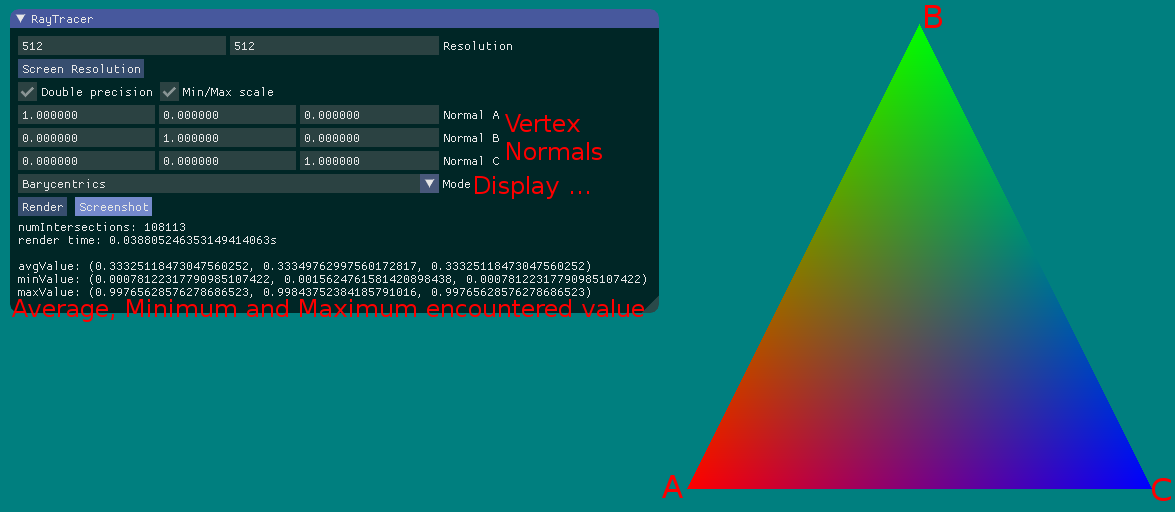
\includegraphics[width=\oneimgwidth\textwidth]{description.png}
	\caption{Barycentrics Visualization}
	\label{fig:desc}
\end{figure}

\FloatBarrier

\subsection{Position Differentials $\dpdx$}

\begin{figure}[htbp] 
	\centering
	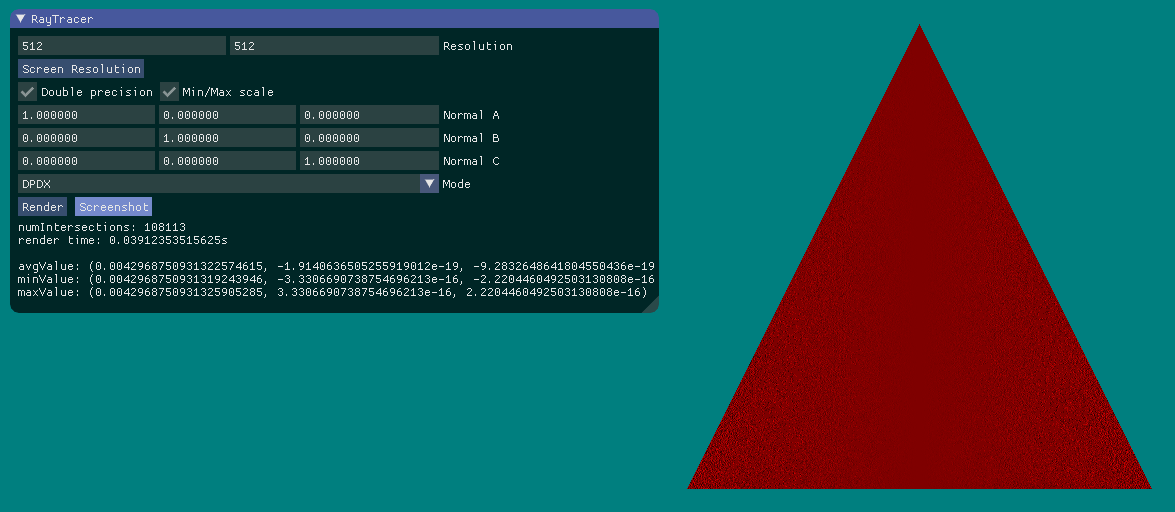
\includegraphics[width=\oneimgwidth\textwidth]{dp/dpdx.png}
	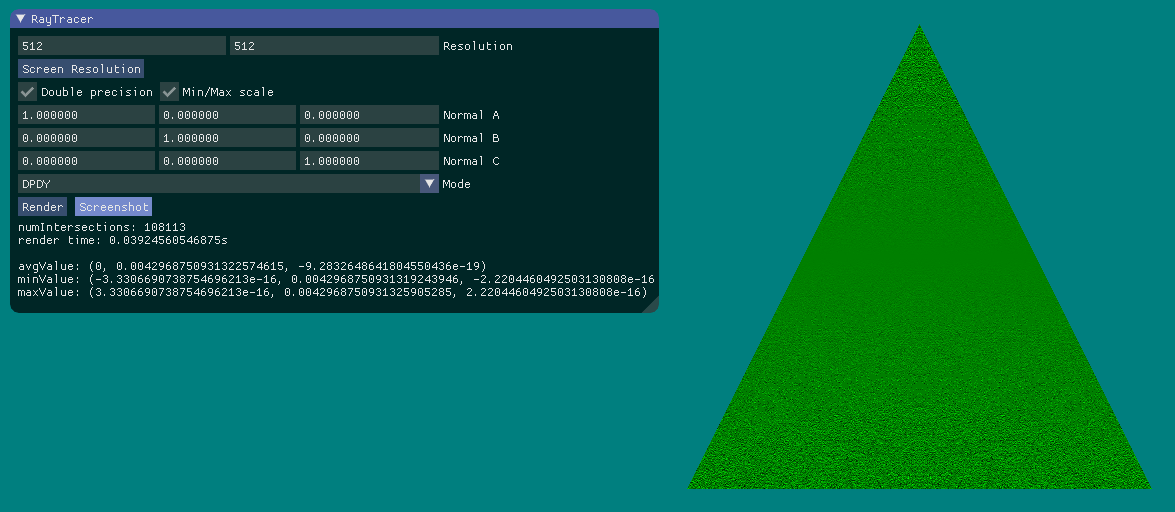
\includegraphics[width=\oneimgwidth\textwidth]{dp/dpdy.png}
	\caption{$\dpdx$ / $\dpdy$}
	\label{fig:dpdx}
\end{figure}

\FloatBarrier

\subsection{Normal Differentials}

\subsubsection{Test}

\begin{figure}[htbp] 
	\centering
	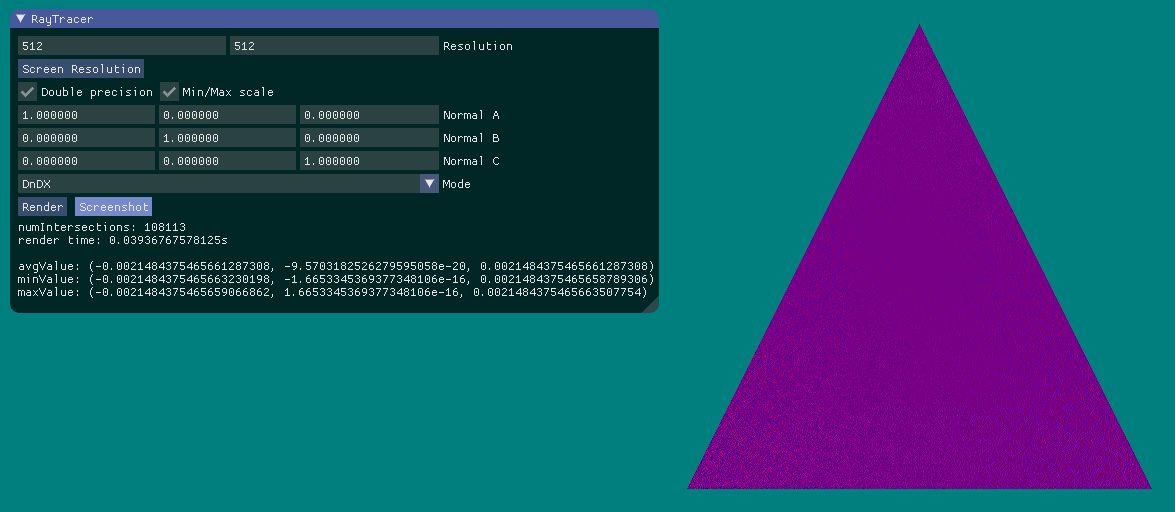
\includegraphics[width=\oneimgwidth\textwidth]{dn/dndx.png}
	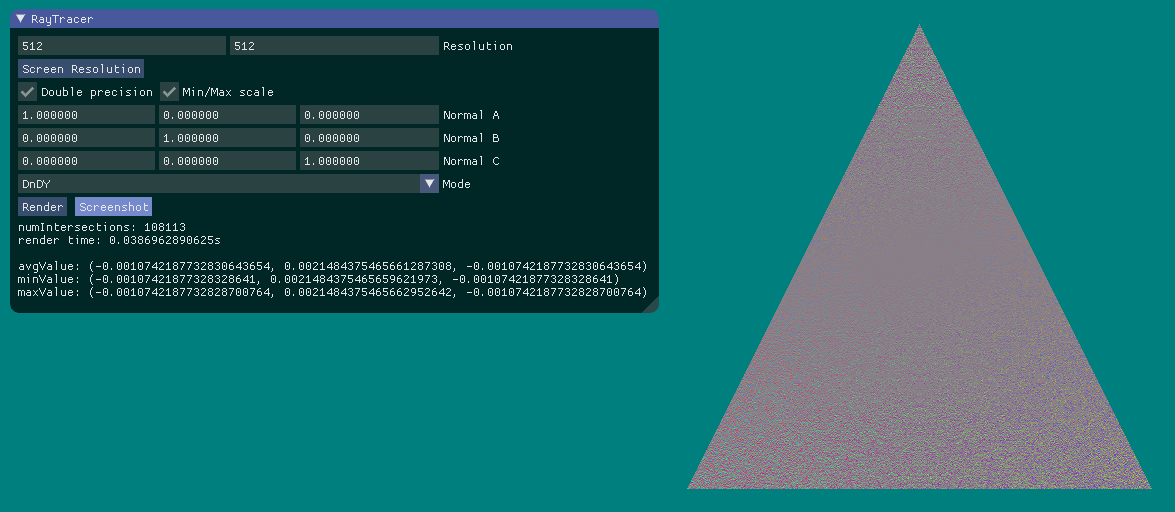
\includegraphics[width=\oneimgwidth\textwidth]{dn/dndy.png}
	\caption{$\dndx$ / $\dndy$}
	\label{fig:dndx}
\end{figure}

\FloatBarrier

\subsubsection{$\dndx$ for $N_A = N_C$ test case}

\begin{equation}
\dndx = \frac{\left(\dpdx\right)_x \left(N_C - N_A\right)}{2}
\end{equation}

\begin{figure}[htbp] 
	\centering
	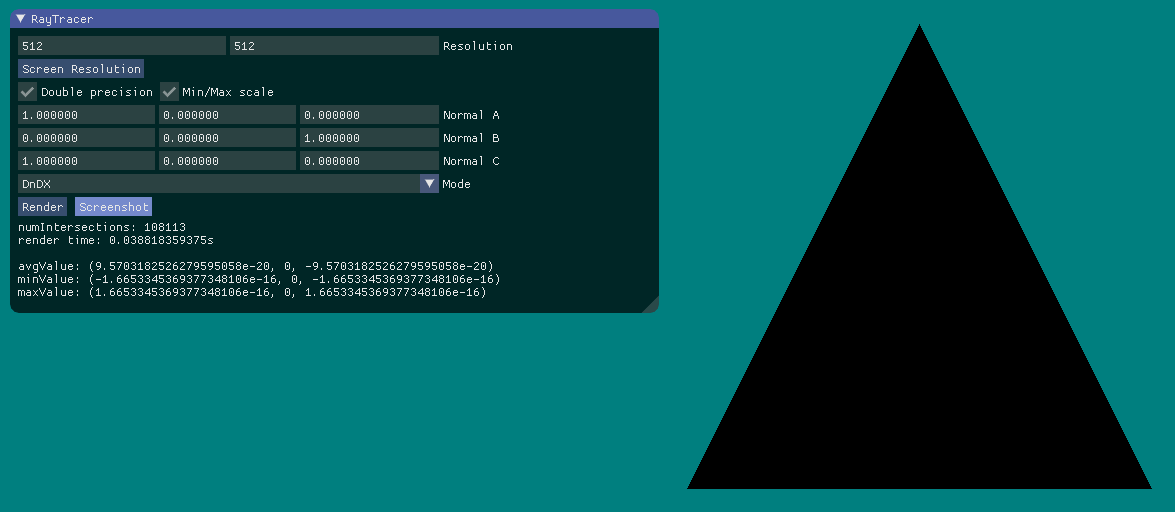
\includegraphics[width=\oneimgwidth\textwidth]{dn/dndx_na_nc_equal.png}
	\caption{$\dndx$ for $N_A = N_C$}
	\label{fig:dndx}
\end{figure}

\FloatBarrier

\subsubsection{$\dndy$ for normals equal test case}

\begin{equation}
\dndy = \frac{\left(\dpdy \right)_y \left(- N_A + 2 N_B - N_C \right)}{4}
\end{equation}

\begin{figure}[htbp] 
	\centering
	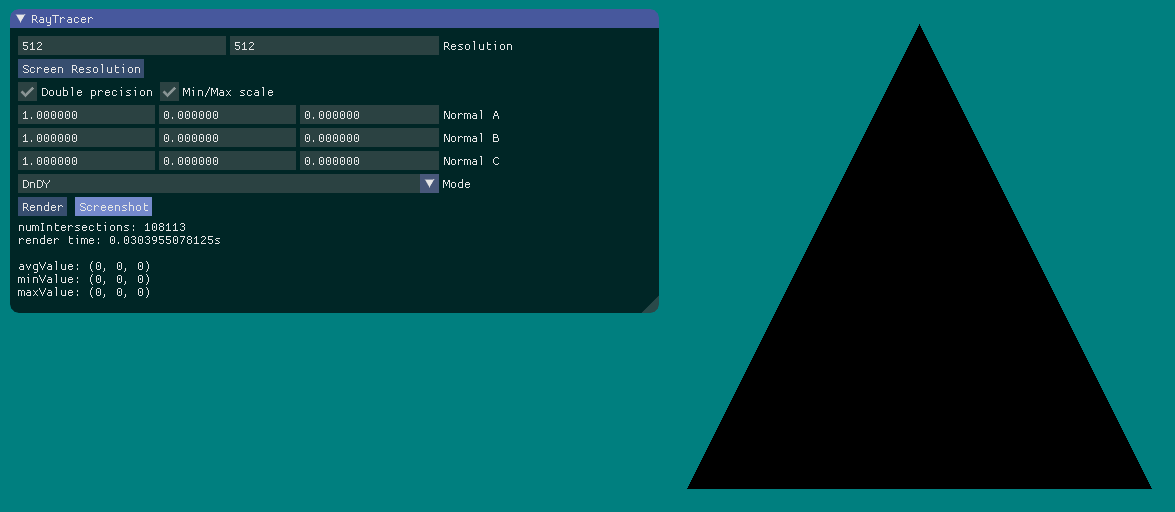
\includegraphics[width=\oneimgwidth\textwidth]{dn/dndy_normals_equal.png}
	\caption{$\dndy$ normals equal}
	\label{fig:dndx}
\end{figure}

\FloatBarrier

\subsubsection{Normal differential by Subtraction}

\begin{equation}
\dndx = n_{P(x) + \dpdx} - n_{P(x)}
\end{equation}

\begin{equation}
\dndy = n_{P(y) + \dpdy} - n_{P(y)}
\end{equation}

\subsubsection{$\dndx$ Differential vs Subtraction}

\begin{figure}[htbp] 
	\centering
	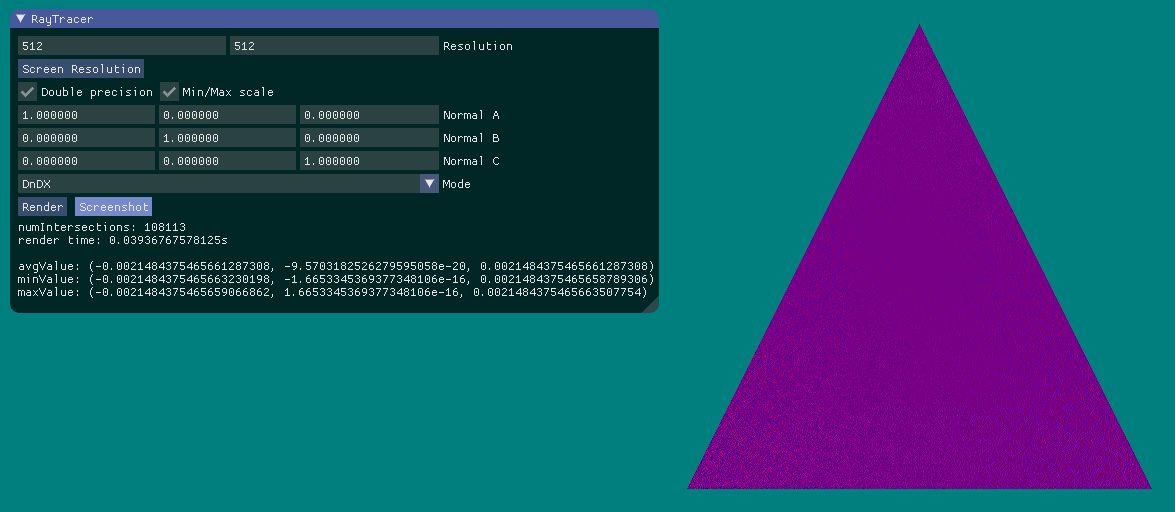
\includegraphics[width=\oneimgwidth\textwidth]{dn/dndx.png}
	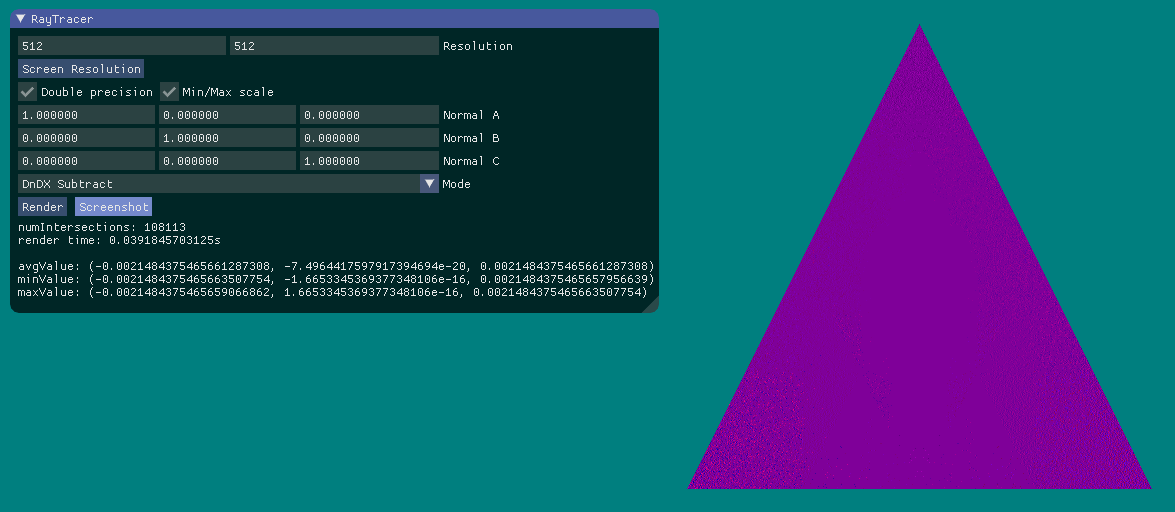
\includegraphics[width=\oneimgwidth\textwidth]{dn/dndx_sub.png}
	\caption{$\dndx$ Differential vs Subtraction}
	\label{fig:dndx}
\end{figure}

\FloatBarrier

\subsubsection{$\dndy$ Differential vs Subtraction}

\begin{figure}[htbp] 
	\centering
	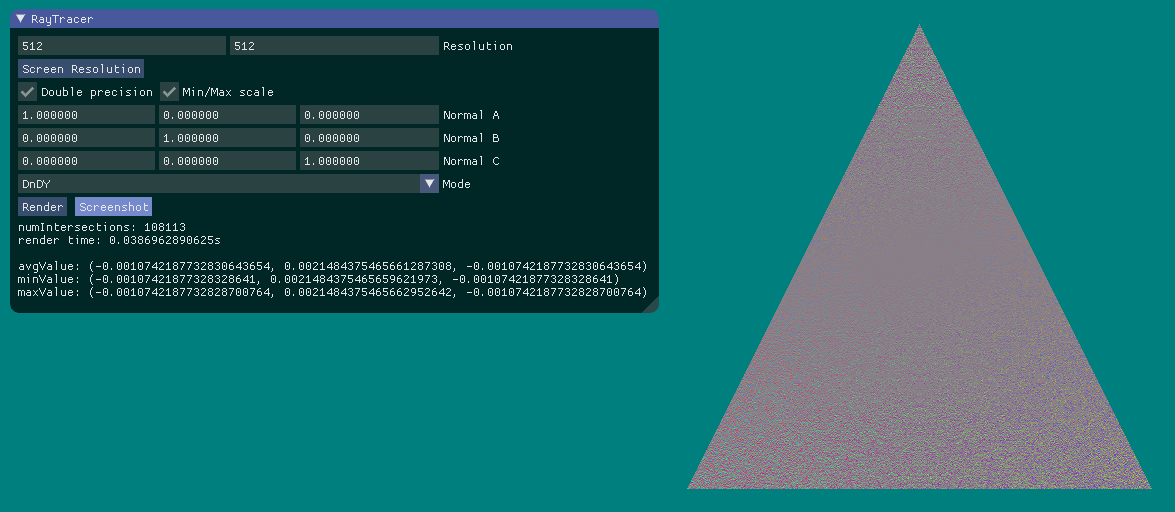
\includegraphics[width=\oneimgwidth\textwidth]{dn/dndy.png}
	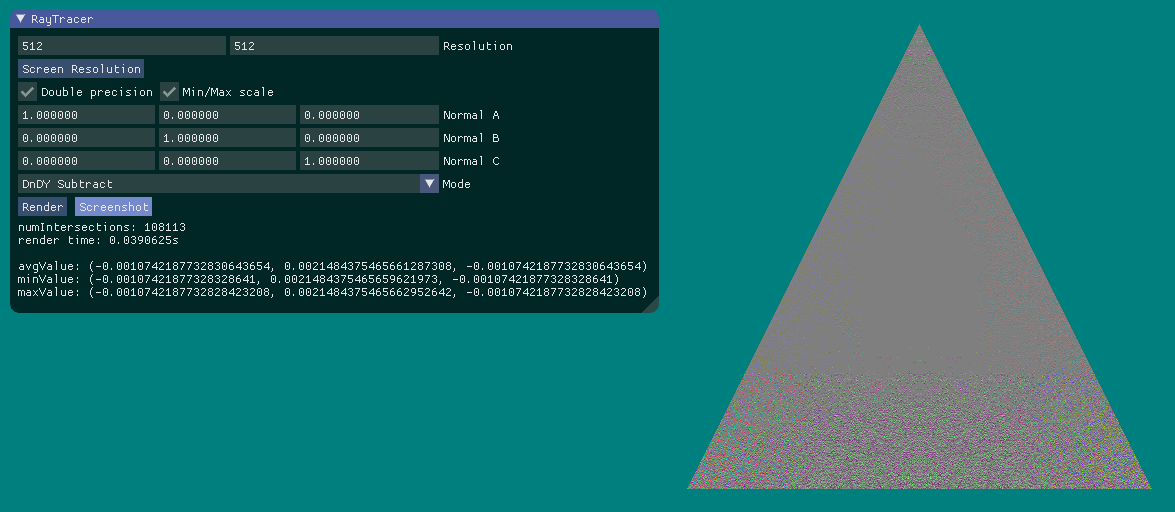
\includegraphics[width=\oneimgwidth\textwidth]{dn/dndy_sub.png}
	\caption{$\dndy$ Differential vs Subtraction}
	\label{fig:dndx}
\end{figure}

\FloatBarrier

\subsubsection{$\dndy$ for $N_A = N_C$ Symmetry test}

\begin{figure}[htbp] 
	\centering
	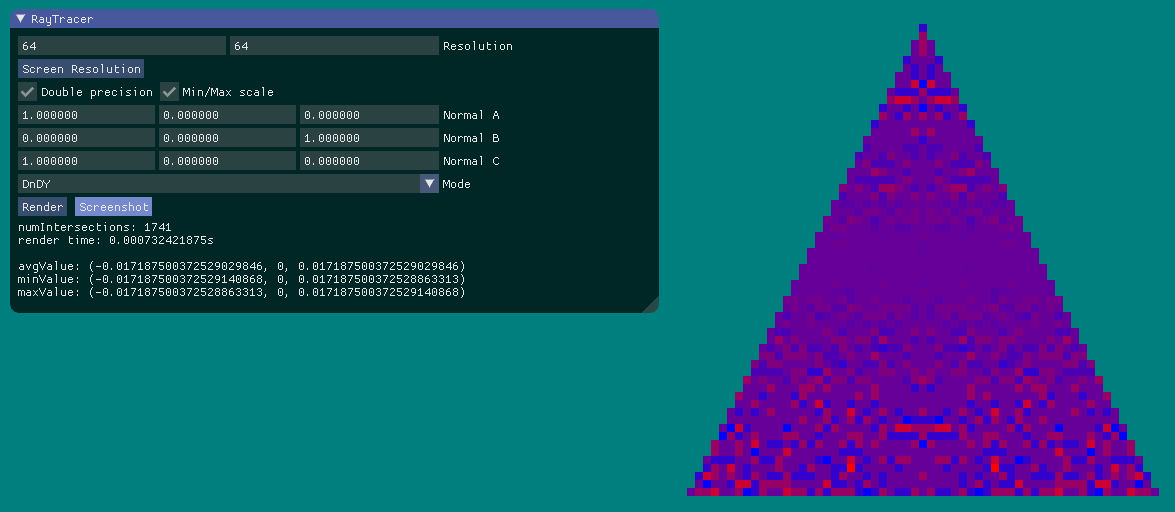
\includegraphics[width=\oneimgwidth\textwidth]{dn/dndy_na_nc_equal_symetry.png}
	\caption{$\dndy$ for $N_A = N_C$ Symmetry test}
	\label{fig:dndx}
\end{figure}

\FloatBarrier

\subsection{Normalized Normal Differentials}

\subsubsection{Test}

\begin{figure}[htbp] 
	\centering
	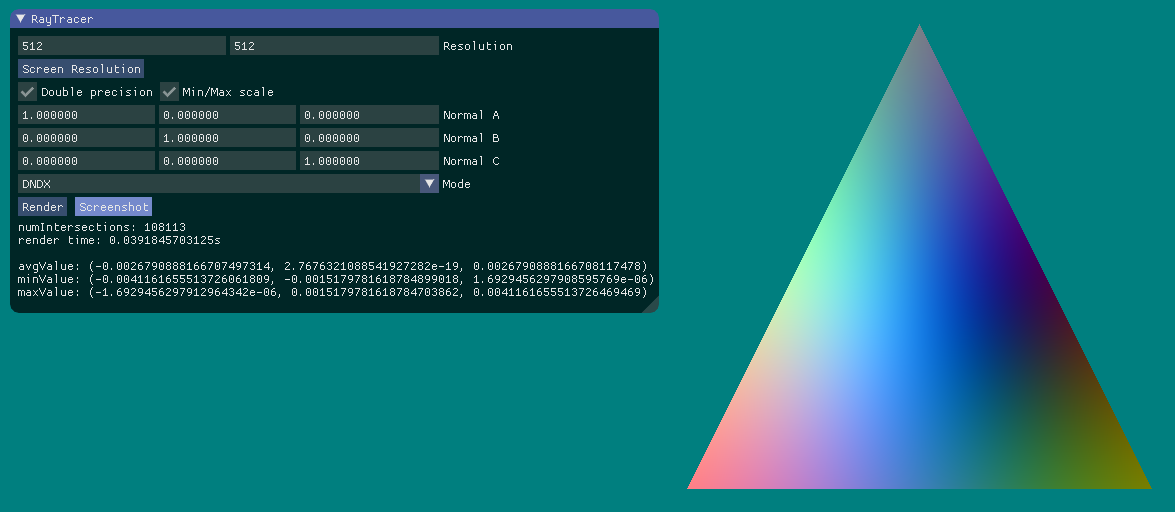
\includegraphics[width=\oneimgwidth\textwidth]{dnn/dnndx.png}
	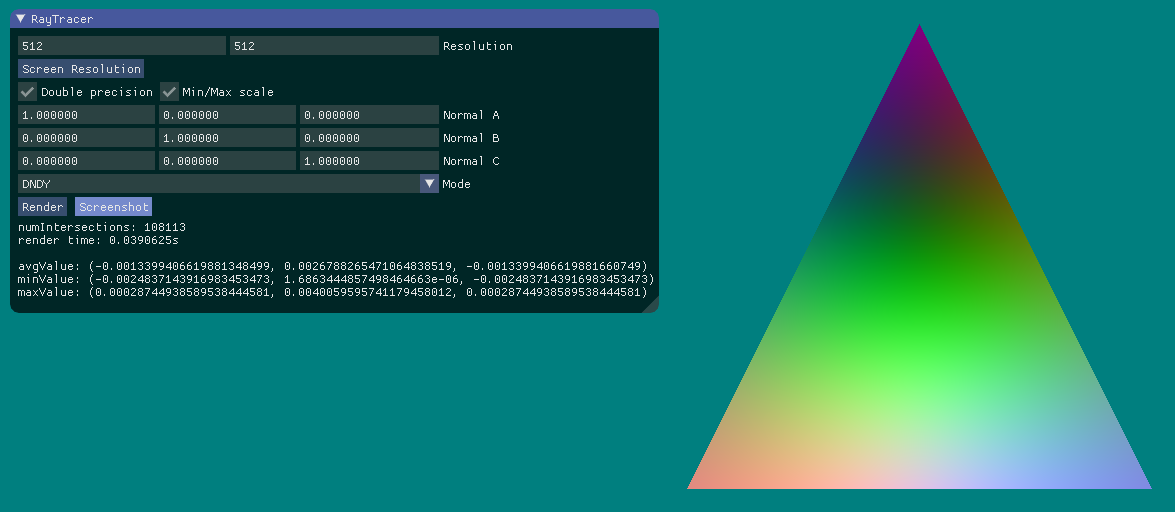
\includegraphics[width=\oneimgwidth\textwidth]{dnn/dnndy.png}
	\caption{$\dnndx$ / $\dnndy$}
	\label{fig:dndx}
\end{figure}

\FloatBarrier

\subsubsection{$\dnndx$ for $N_A = N_C$ test case}

\begin{figure}[htbp] 
	\centering
	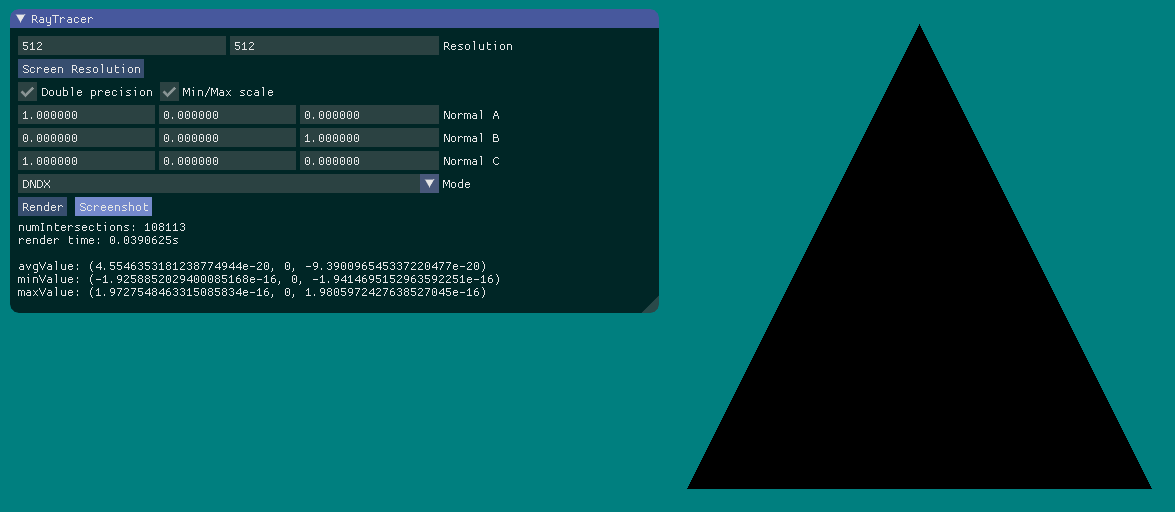
\includegraphics[width=\oneimgwidth\textwidth]{dnn/dnndx_na_nc_equal.png}
	\caption{$\dnndx$ for $N_A = N_C$ test case}
	\label{fig:dndx}
\end{figure}

\FloatBarrier

\subsubsection{$\dnndy$ for normals equal}

\begin{figure}[htbp] 
	\centering
	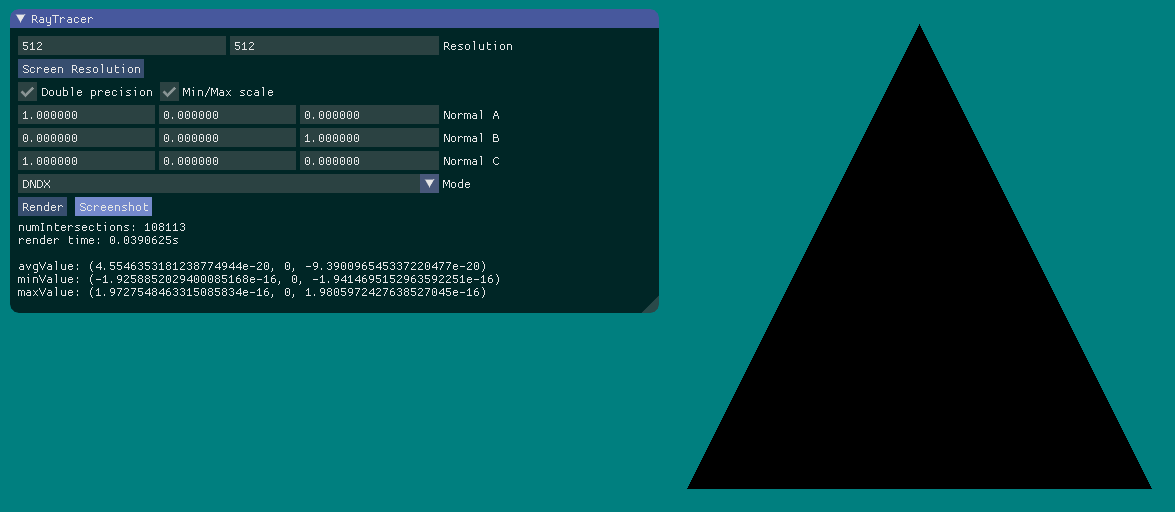
\includegraphics[width=\oneimgwidth\textwidth]{dnn/dnndx_na_nc_equal.png}
	\caption{$\dnndy$ for normals equal}
	\label{fig:dndx}
\end{figure}

\FloatBarrier

\subsubsection{Normalized Normal differential by Subtraction}

\begin{equation}
\dnndx = N_{P(x) + \dpdx} - N_{P(x)}
\end{equation}

\begin{equation}
\dnndy = N_{P(y) + \dpdy} - N_{P(y)}
\end{equation}

\subsubsection{$\dnndx$ Differential vs Subtraction}

\begin{figure}[htbp] 
	\centering
	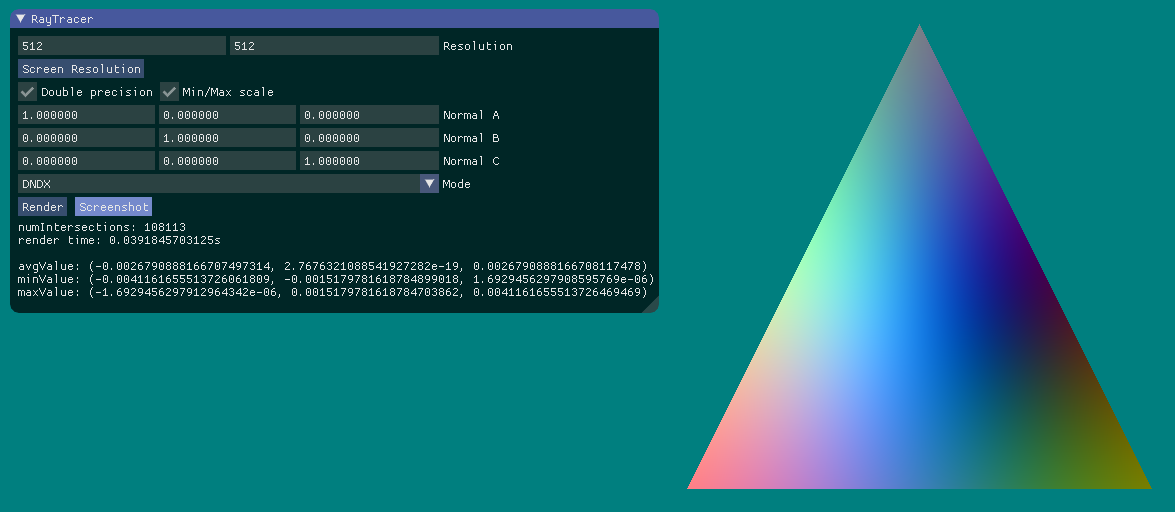
\includegraphics[width=\oneimgwidth\textwidth]{dnn/dnndx.png}
	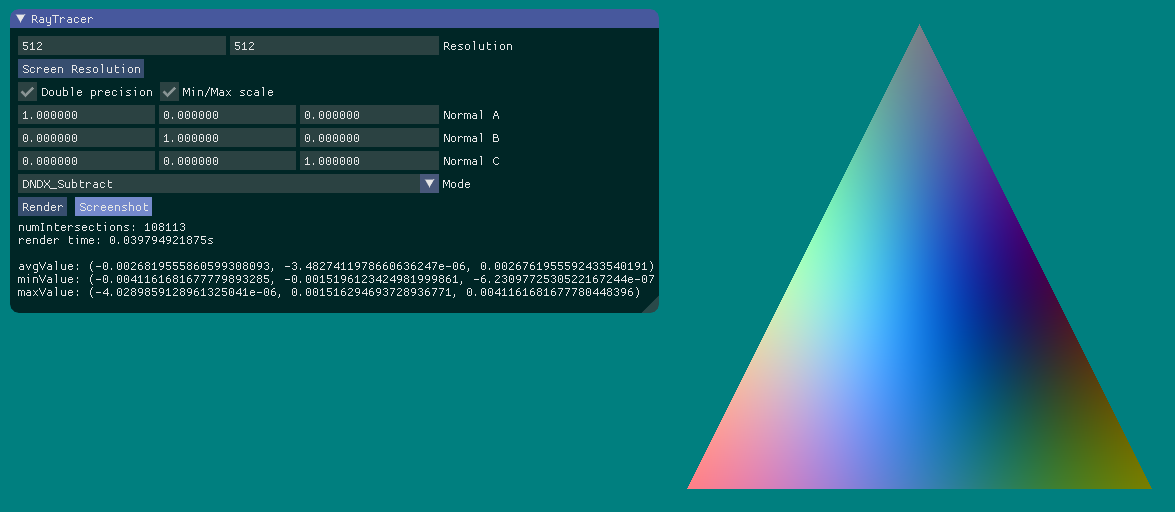
\includegraphics[width=\oneimgwidth\textwidth]{dnn/dnndx_sub.png}
	\caption{$\dnndx$ Differential vs Subtraction}
	\label{fig:dndx}
\end{figure}

\FloatBarrier

\subsubsection{$\dnndy$ Differential vs Subtraction}

\begin{figure}[htbp] 
	\centering
	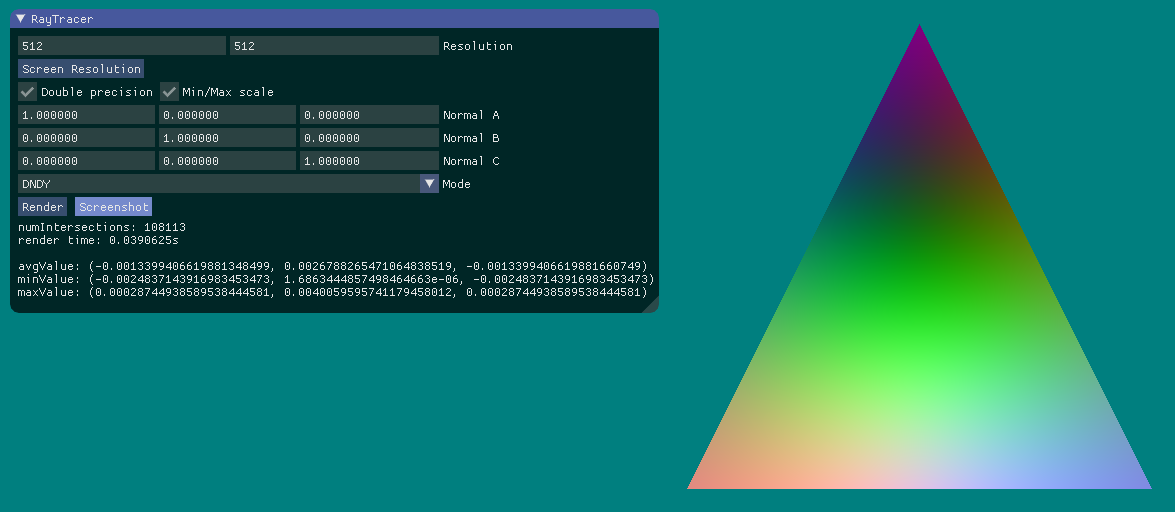
\includegraphics[width=\oneimgwidth\textwidth]{dnn/dnndy.png}
	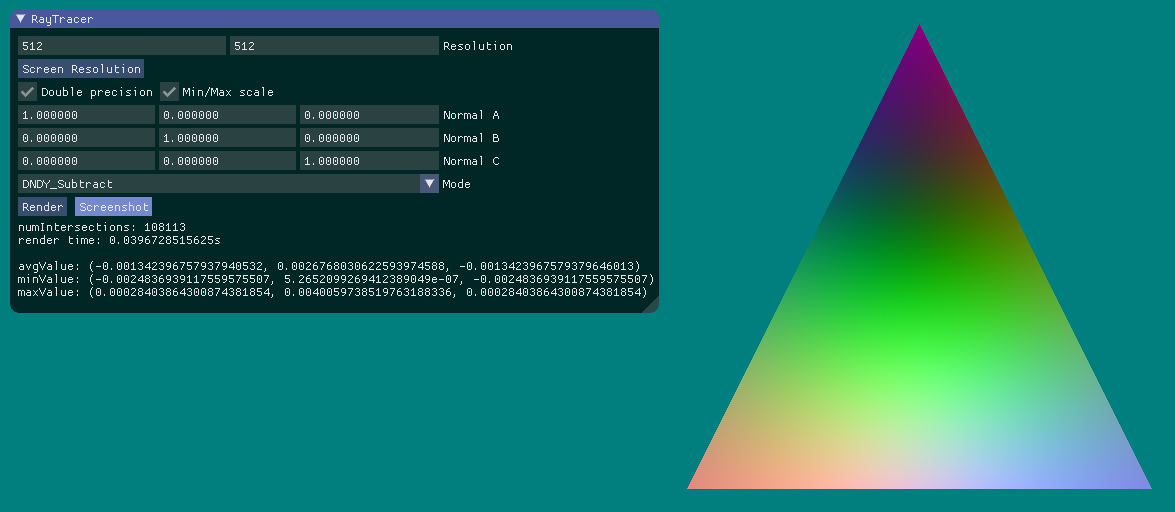
\includegraphics[width=\oneimgwidth\textwidth]{dnn/dnndy_sub.png}
	\caption{$\dnndy$ Differential vs Subtraction}
	\label{fig:dndx}
\end{figure}

\FloatBarrier

\subsubsection{$\dnndx$	$N_A$ and $N_C$ facing away}

\begin{figure}[htbp] 
	\centering
	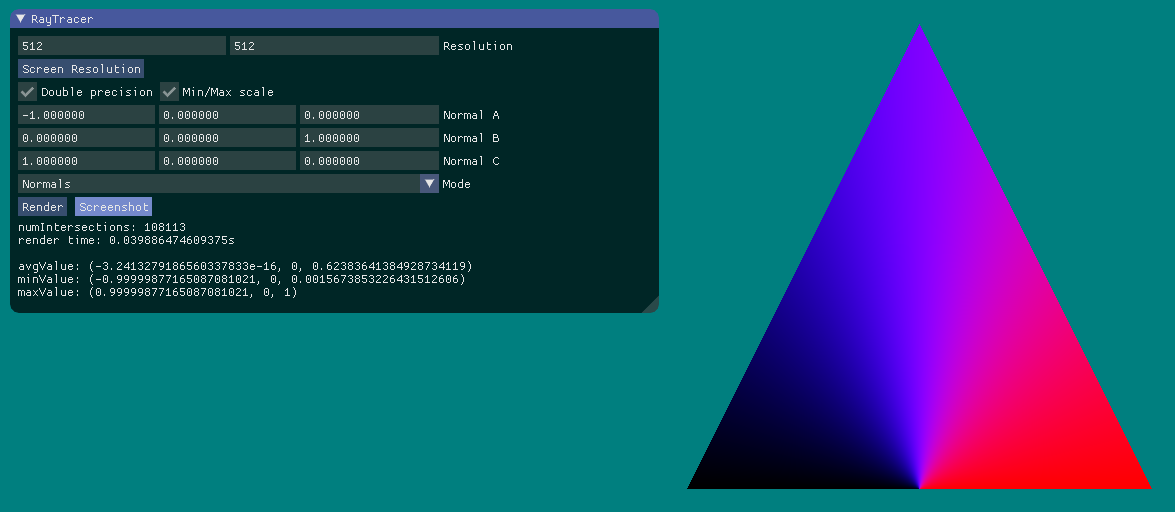
\includegraphics[width=\oneimgwidth\textwidth]{dnn/normals_na_nc_facing_away.png}
	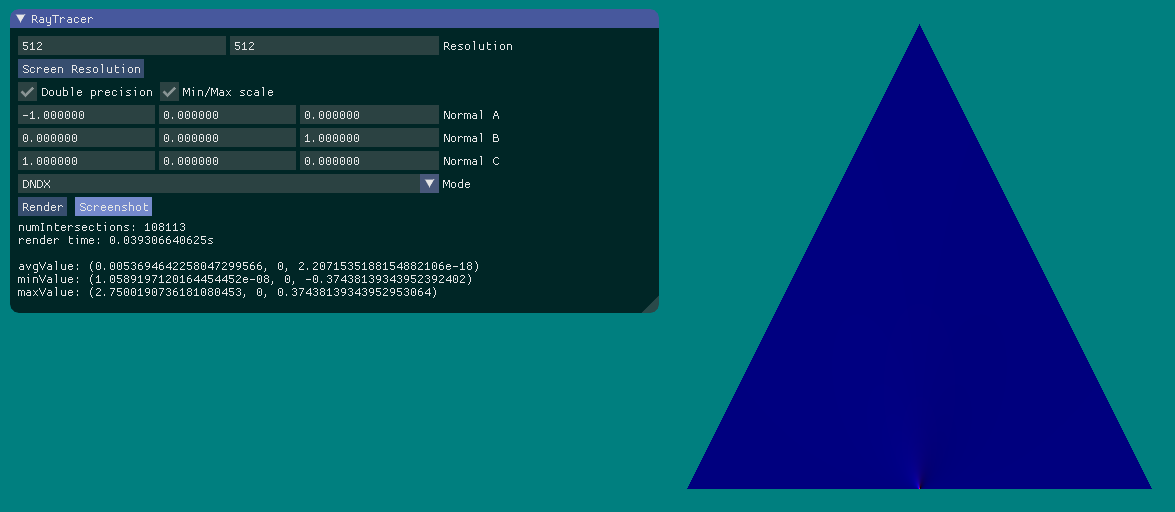
\includegraphics[width=\oneimgwidth\textwidth]{dnn/ddndx_na_nc_facing_away.png}
	\caption{$\dnndx$ Normals facing away Normal Visualization vs Differential}
	\label{fig:dndx}
\end{figure}

\begin{figure}[htbp] 
	\centering
	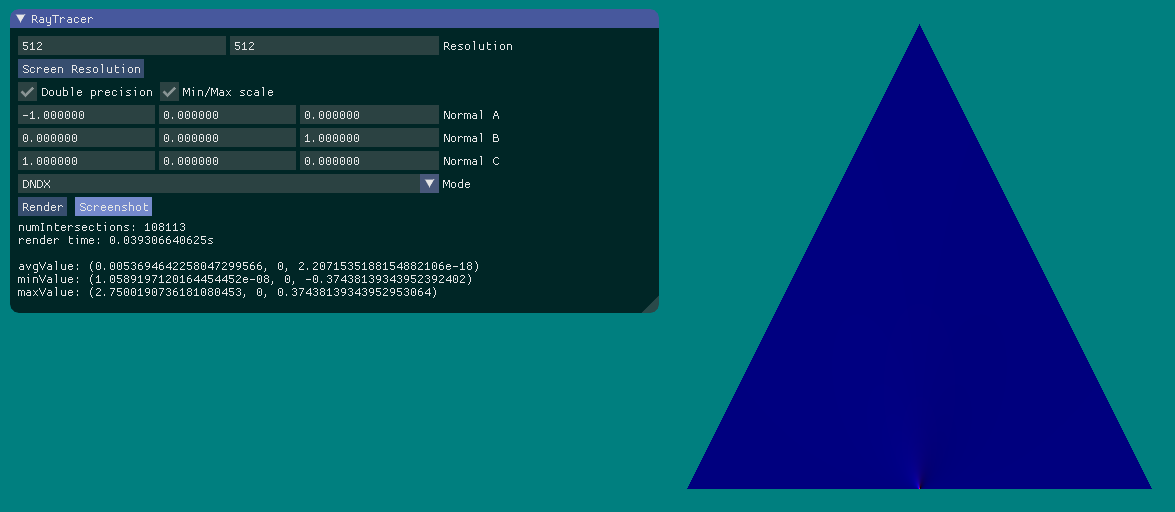
\includegraphics[width=\oneimgwidth\textwidth]{dnn/ddndx_na_nc_facing_away.png}
	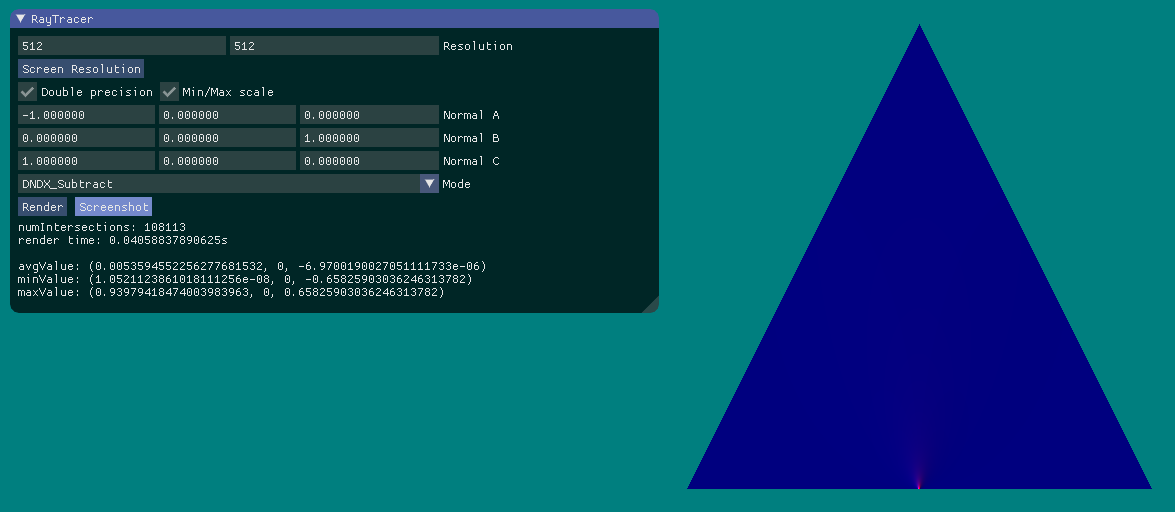
\includegraphics[width=\oneimgwidth\textwidth]{dnn/dnndx_sub_na_nac_facing_away.png}
	\caption{$\dnndx$ Normals facing away Differential vs Subtraction}
	\label{fig:dndx}
\end{figure}

\end{document}